\section{High-level Design}\label{sec:tern-design}


Our design of \tern adheres to the following goals:

\begin{enumerate}

\item {\bf Backward compatibility}.  We design \tern for general
  multithreaded programs because of their dominance in parallel programs
  today and likely tomorrow.  We design \tern to run in user-space and on
  commodity hardware to ease deployment.

\item {\bf Stability}.  We design \tern to bias multithreaded programs
  toward repeating their past, familiar schedules, instead of venturing
  into unfamiliar ones.

\item {\bf Efficiency}.  We design \tern to be efficient because it
  operates during the normal executions of programs, not replayed
  executions.

\item {\bf Best-effort determinism}.  We design \tern to make threads
  deterministic, but we sacrifice determinism when it contradicts the
  preceding goals.

\end{enumerate}

The remaining of this section presents \tern's architecture
(\S\ref{sec:arch}), workflow (\S\ref{sec:example}), deployment scenarios
(\S\ref{sec:offline}), and limitations (\S\ref{sec:limit}).

%% We aim for best-effort determinism because true determinism has a high
%% cost (\S\ref{sec:schedule-constraints}).  Moreover, input nondeterminism
%% cannot be fully eliminated anyway, so we may as well tolerate some
%% scheduling nondeterminism, following the end-to-end
%% argument~\cite{saltzer:end2end:tocs}.

\subsection{Architecture} \label{sec:arch}

\begin{figure}[t]
\begin{center}
\includegraphics[width=0.48\textwidth]{tern/figures/overview.eps}
\end{center}
\caption{\emph{\tern architecture.} Its components are shaded.}
\label{fig:overview}
\end{figure}

Figure~\ref{fig:overview} shows the architecture of \tern and its five
components: \emph{instrumentor}, \emph{schedule cache}, \emph{proxy},
\emph{replayer}, and \emph{memoizer}.  To use \tern, developers first
annotates their application by marking the input data that may affect
synchronization operations.  They then compile their program with the
\emph{instrumentor}, which intercepts standard synchronization operations
such as \v{pthread\_mutex\_lock()} so that at runtime \tern can control
these operations.  (We describe additional annotations and
instrumentations that \tern needs in \S\ref{sec:annotations}).  The
instrumentor runs as a plugin to LLVM~\cite{llvm}, requiring no
modifications to the compiler.
%  and avoiding the overhead of dynamic instrumentation.

% overhead, %actually not much.

%% The \emph{instrumentor} runs as a compiler plugin to avoid dynamic
%% instrumentation overhead.  It takes two types of developer annotations:
%% (1) the portions of input data that may affect scheduling and (2) custom
%% synchronizations (\eg, atomic operations) which \tern includes in the
%% synchronization orders it memoizes.  It intercepts these and other
%% synchronization operations to call into the replayer and the memoizer.  It
%% also computes the set of branch statements these operations depend upon
%% for the memoizer to simplify input constraints (\S\ref{sec:slicing}).

The \emph{schedule cache} stores all memoized schedules and their input
constraints.  This cache can be marshalled to disk and read back upon
program start, so that it need not be repopulated.
Each memoized schedule
is conceptually a tuple $\langle C, S \rangle$, where $S$ is a
synchronization order and $C$ is the set of input constraints required to reuse
$S$. (We explain the actual representation in
\S\ref{sec:track-constraints}).

At runtime, once an input $I$ arrives, the \emph{proxy} intercepts the
input and queries the schedule cache for a constraint-schedule tuple
$\langle C_i, S_i \rangle$ such that $I$ satisfies $C_i$.  On a cache hit,
the proxy lets the \emph{replayer} run the program on input $I$ and enforce
schedule $S_i$.  On a cache miss, it lets the \emph{memoizer} run the
program on input $I$ to memoize a new schedule.

During a memoization run, the memoizer records all synchronization
operations into a schedule $S$.  It also computes $C$, the input
constraints for reusing $S$, via symbolic execution~\cite{klee:osdi08}.
The basic idea of symbolic execution is to track the outcomes of branches
that observe symbolic data, in our case, the data marked by developers as
affecting synchronizations.  Once the memoization run ends, the set of
branch outcomes we collected describes the input constraints needed to reuse
the memoized schedule.
%% To reduce the proxy's overhead of checking constraints, the
%% memoizer simplifies $C$ by removing constraints irrelevant to $S$.  

For determinism, the memoizer can optionally check a memoization run for
data races.  If it detects no races, it simply stores $\langle C, S
\rangle$ into the schedule cache.  Otherwise, it can discard the memoized
schedule and rerun the program with a different scheduling algorithm to
memoize another schedule.

The proxy performs an additional task for server programs to reduce input
timing nondeterminism and to reuse schedules for these programs.
Specifically, it buffers the requests of a server into a window with
a fixed size.
When the window becomes full, or remains partial for a predefined timeout,
\tern runs the server to process the window as if the server were a batch
program.  It then lets the server quiesce before moving to the next window to
avoid interference between windows.

% If the schedule turns out 

%When a new input arrives, \tern searches this schedule cache and reuses an
%existing schedule if possible, instead of creating a new schedule.
%\tern shares similarity with deterministic replay systems because it
%records and ``replays'' schedules.  However, unlike deterministic replay
%systems, \tern attempts to replay recorded schedules on different inputs.

%A schedule and its constraints collected by the instrumentation code are
%stored in \tern's schedule cache.  

% (\S\ref{sec:cache} presents the real data structures we use to speed up
% lookup of the schedule cache.)



\subsection{Workflow and An Example} \label{sec:example}

\begin{figure}[t]
\centering \tiny \lgrindfile{tern/code/pbzip2.cpp.lineno}
\caption{\small Simplified \pbzip code.}
\label{fig:pbzip2}
\end{figure}

\begin{figure}[t]
\centering
\begin{minipage}[c]{.8\linewidth}
\tiny \lgrindfile{tern/code/pbzip2-sync-order.cpp}
%\includegraphics[width=.4\textwidth]{figures/pbzip2-sync-order.eps}
\end{minipage}
\caption{\small Synchronization order of a \pbzip run.}
\label{fig:pbzip2-sync-order}
\end{figure}

\begin{figure}[t]
\centering
\begin{minipage}[c]{0.4\linewidth}
\tiny \lgrindfile{tern/code/pbzip2-constraints.cpp}
\end{minipage}
\caption{\small Input constraints of a \pbzip run.}
\label{fig:pbzip2-constraints}
\end{figure}

We illustrate how \tern works using \pbzip as an example.
Figure~\ref{fig:pbzip2} shows the simplified code of \pbzip.  Variables
\v{nthread} and \v{nblock} affect synchronizations, so developers mark
them by calling the \tern-provided method \v{symbolic()} (line 3 and line 4).  This
code spawns \v{nthread} worker threads, splits the file into \v{nblock}
blocks, and compresses them in parallel by calling \v{compress()}.  To
coordinate the worker threads, it uses a synchronized work list. (Note \tern tracks
low-level synchronizations such as pthread primitives; we use a work list
here only for clarity.)

Suppose we run \pbzip with two threads on a two-block file.  Suppose the
schedule cache is empty and \tern runs the memoizer to memoize a new
schedule.  As \pbzip runs, \tern controls and records the synchronization
operations (line 9 and line 14).  It also tracks the outcomes of branch
statements that observe symbolic data (line 5 and line 7).  At the end of the
run, \tern records a schedule as shown in
Figure~\ref{fig:pbzip2-sync-order}.  It also collects constraints as shown
in Figure~\ref{fig:pbzip2-constraints}, which simplify to $nthread=2
\wedge nblock=2$.\footnote{Although in this example the constraints are
  collected from one thread, \tern can actually collect constraints from
  multiple threads.}  It stores the schedule and the input constraints
into the schedule cache.

If we run \pbzip again with two threads on a different two-block file,
\tern will check if variable \v{nthread} and \v{nblock} satisfy any set of
constraints in the schedule cache.  In this case, \tern will succeed.  It
will then reuse the schedule (Figure~\ref{fig:pbzip2-sync-order}) to
compress the file, even though the file data may differ completely.

%The synchronization order in this sub-figure can be reused to compress
%many different files, as long as the number of threads and the number of
%blocks remain the same, regardless of the file contents.


%% \begin{figure*}[t]
%% \centering
%% \includegraphics[width=.9\textwidth]{figures/pbzip2-sync-order.eps}
%% \caption{{\em pbzip2 example}.  Sub-figure (a) shows the simplified pbzip2 code.
%%   Sub-figure (b) shows the synchronization order of a run of pbzip2 with
%%   two threads on a two-chunk file; the arrows (in red) depict the
%%   execution order.  Sub-figure (c) shows the input constraints of the run;
%%   the branches taken are solid arrows (in red) and those not taken are
%%   dashed.}
%% \label{fig:pbzip2}
%% \end{figure*}

\subsection{Deployment Scenarios} \label{sec:offline}

We anticipate three ways users may deploy \tern to make their programs
stable and deterministic.

\para{Schedule-carrying code.} Developers pre-populate a cache of correct,
representative schedules on typical workloads, then ship their program
with the cache hardwired and marked read-only.

\para{Online memoization.}  Users can turn on memoization at their local
sites so that \tern can memoize schedules as the programs run on real
inputs.

\para{Shadow memoization.} Since tracking input constraints is slow, users
can configure \tern to memoize schedules asynchronously.  Specifically, for
an input that misses the schedule cache, the proxy runs the program as is,
while forwarding a copy of the input to the memoizer.

\para{} Each deployment mode has pros and cons.  The first mode makes a
program stable and deterministic across different sites, but may react
poorly to site-specific workloads.  The second mode updates the schedule
cache based on site-specific workloads, but may be slow because
memoization runs tend to be slow.  The last approach avoids the slowdown,
but allows a program to run nondeterministically when an input misses the
schedule cache.  For server programs with high performance requirements,
we recommend the first and the third modes.

% Based on these pros and cons, we recommend the first and second mode for
% batch programs, and the first and third mode for server programs which
% tend to have high performance demand.

%% By decoupling execution and memoization, we enjoy similar
%% benefits as previous work~\cite{decouple:usenix08}.

%% \tern can operate in both offline and online mode.  In offline mode,
%% developers pre-populate a cache of correct, representative schedules by
%% running their program against representative workloads prior to shipping
%% their program.  They then ship their program together with the schedule
%% cache hardwired into the program and marked readonly.  This mode makes
%% program more deterministic and stable across different sites because each
%% site has the same schedule cache.  This mode is the default mode of \tern.

%% In online mode, \tern updates the schedule cache as a program runs on real
%% inputs.  This mode may react better to the diverse workloads at users
%% sites.  However, tracking constraints is expensive because it requires
%% instrumenting memory accesses and branch instructions~\cite{klee:osdi08}.
%% (This slowdown is not a big problem for offline mode.) \tern addresses this
%% problem by memoizing schedules asynchronously.  For each input that does
%% not hit the schedule cache, \tern lets the program process the input as is
%% without tracking any constraints.  Meanwhile, it runs a shadow version of
%% the program on the same input and tracks constraints.  To avoid
%% interfering the actual run, \tern sandboxes the shadow run by crudely
%% forking a process and dropping all file and network output. (Better
%% sandboxes can of course be built.)

\subsection{Limitations} \label{sec:limit}

% We discuss \tern's limitations in this subsection.

\para{Determinism.} \tern aims for best-effort determinism for reasons
discussed in \S\ref{sec:define-schedule}.  If \tern is unable to find a
race-free schedule for an input, the run may be nondeterministic.  We
foresee several strategies to handle this corner case while adhering to
the other goals of \tern.  For instance, we can instrument the program to
fix the detected races or apply one of the existing \dmt algorithms to
resolve the races deterministically.  The advantage of combining these
techniques with \tern is that we apply these expensive techniques only to a
small portion of schedules, and use \tern to efficiently handle the common
case.  We leave these ideas for future work.

%%\todo{mismatch assumption and application}

\para{Applicability.} We anticipate our approach will work well for many
programs/workloads as long as (1) they can benefit from determinism and
stability, (2) their constraints can be tracked by \tern, (3) their
schedules can be frequently reused, and (4) if windowing is needed, their
inputs can be buffered.  For programs/workloads that
violate these assumptions, \tern may work poorly.  These programs/workloads
may include parallel simulators that require nondeterminism for
statistical results, GUI programs that cannot buffer user actions for
latency reasons, randomly generated workloads that prevent schedule
reuses, and programs whose schedules depend on floating point inputs
(which cannot be tracked by \tern's underlying symbolic execution engine).

%At an implementation level, the symbolic engine we use does not handle
%floating points.

\para{Manual annotation.} \tern requires manual annotations.  However, this
annotation overhead tends to be small.  (See \S\ref{sec:slicing} for how
\tern reduces this overhead and \S\ref{sec:ease-of-use} for an evaluation
of this overhead).  This overhead may be further reduced using simple static analysis.
% a concurrently published technique~\cite{syncfinder:osdi10}, which we
% have not yet implemented.



\section{Interface}  \label{sec:annotations}

\begin{table*}[t]
\small
\centering
\begin{tabular}{lcp{4.1in}}
{\bf Annotations} & {\bf Inserted by} &  {\bf Semantics} \\

\hline

\multirow{2}{*}{symbolic(\emph{data}, \emph{len})} &
\multirow{2}{*}{Developer} & Marks data that may affect
schedules.  The memoizer tracks constraints on this data.  The replayer
checks this data against the memoized constraints. \\ \hline

begin\_task() & \multirow{2}{*}{Developer} & \multirow{2}{4.1in}{Mark the
  beginning and end of a logical task.  Often used to divide the
  executions of threads in a pool into separate tasks
  (\S\ref{sec:window}).  }\\

end\_task() & & \\

\hline

lock\_wrapper(\emph{l}) & Developer & \multirow{2}{4.1in}{Synchronization
  wrappers.  The memoizer intercepts these operations for memoizing
  schedules, and the replayer intercepts them for reusing schedules.  } \\

unlock\_wrapper(\emph{l}) & or \tern & \\

% up\_wrapper(\emph{s}) & & \\

% down\_wrapper(\emph{s}) & & \\

\hline

before\_blocking() & \multirow{2}{*}{\tern} &
\multirow{2}{4.1in}{Inserted before and after blocking system calls.  The
  memoizer logs the order of these calls. The replayer opportunistically
  enforces the same order of these calls.}\\

after\_blocking() & & \\

\end{tabular}
\caption{\small {\em \tern interface.}  Some annotations are inserted by
  developers, and others are inserted by the instrumentor, indicated by
  Column {\bf Inserted By}.  Both the memoizer and the replayer use this
  interface, but they implement this interface differently
  (\S\ref{sec:batch}).} \label{tab:interface}
\end{table*}

Table~\ref{tab:interface} shows \tern's annotation interface which
developers and the instrumentor use to annotate multithreaded programs.
The annotations fall into four categories: (1) \v{symbolic()} for marking
data that may affect schedules; (2) task boundary annotations for marking
the beginning and end of logical tasks, in case threads get reused for
different logical tasks (\S\ref{sec:window}); (3) wrappers to
synchronization operations (more examples in the next paragraph); and (4) hook
functions inserted around blocking system calls, which \tern memoizes
because blocking systems calls are natural scheduling points.

Currently \tern hooks 28 pthread operations (\eg, \v{pthread\_mutex\_lock()},
\v{pthread\_create()}, and \v{pthread\_cond\_wait()}).  It also handles
common atomic operations such as \v{atomic\_dec()} and \v{atomic\_inc()}.
It hooks eight blocking system calls (\eg, \v{sleep()}, \v{accept()},
\v{recv()}, \v{select()}, and \v{read()}). These hooks are sufficient to
run the programs evaluated, and we can easily add more.

Developers manually insert annotations in the first two categories.  They
also annotate custom synchronizations (\eg, custom spin locks).  \tern's
instrumentor automatically hooks standard synchronization and blocking
system calls.  These annotations allow \tern's memoizer and replayer to run
as ``parasitic'' user-space schedulers that oversee the scheduling
decisions of the OS and synchronization library, requiring no
modifications to either.

% This transparent approach is used in previous
% systems~\cite{r2:osdi,modist:nsdi09,musuvathi:chess:osdi08} as well.

% signal handlers and asynchronous I/O completion.?


%% pthreads operations
%%
%% pthread\_mutex\_lock()
%% pthread\_mutex\_trylock()
%% pthread\_mutex\_unlock()

%% sem\_wait()
%% sem\_trywait()
%% sem\_timedwait()
%% sem\_post()

%% pthread\_barrier\_wait()

%% pthread\_cond\_signal()
%% pthread\_cond\_broadcast()
%% pthread\_cond\_wait()
%% pthread\_cond\_timedwait()

%% ppthread\_create()
%% pthread\_exit()
%% pthread\_join()

%% system calls

%% sleep()
%% usleep()
%% nanosleep()
%% sched_yield

%% read()
%% accept()
%% recv()
%% select()
